% 《物理实验报告模板.tex》的共同版式；所有实验模板均载入本文件。
\documentclass[UTF8,a4paper,10pt,fontset=fandol]{ctexart}
\usepackage[left=3.175cm,right=3.175cm,top=2.54cm,bottom=2.54cm]{geometry}
\usepackage{graphicx,tikz,pgfplots,needspace,adjustbox,booktabs,fancyhdr,lastpage,amsmath,amssymb,array,tabularx,longtable}
\pgfplotsset{compat=1.18}
\setlength{\parindent}{0pt}
\setlength{\parskip}{2pt}
\setlength{\headheight}{18pt}
\linespread{1}
\newcommand{\SetField}[2]{\expandafter\def\csname reportfield@#1\endcsname{#2}}
\makeatletter
\newcommand{\Field}[2][1.35cm]{%
  \ifcsname reportfield@#2\endcsname
    \expandafter\ifx\csname reportfield@#2\endcsname\@empty
      \underline{\makebox[#1]{\strut}}%
    \else\csname reportfield@#2\endcsname\fi
  \else\underline{\makebox[#1]{\strut}}\fi}
\makeatother
\newcommand{\MathField}[2][1.35cm]{%
  \ifcsname reportfield@math_#2\endcsname
    \csname reportfield@math_#2\endcsname
  \else\text{\Field[#1]{#2}}\fi}
\newcommand{\coverfield}[2]{%
  \noindent{\heiti\fontsize{18pt}{48pt}\selectfont
  \makebox[3.3cm][l]{#1}\underline{\makebox[8.8cm][c]{\Field[0pt]{#2}}}\par}}
\newcommand{\bindingline}[1][2.85]{%
  \begin{tikzpicture}[remember picture,overlay]
    \foreach \i in {0,...,38}{%
      \pgfmathsetmacro{\bindingy}{-#1-0.52*\i}%
      \ifnum\i=13\relax
        \node[inner sep=0pt] at ([xshift=1.05cm,yshift=\bindingy cm]current page.north west) {\songti\fontsize{10.5pt}{10.5pt}\selectfont 装};
      \else\ifnum\i=19\relax
        \node[inner sep=0pt] at ([xshift=1.05cm,yshift=\bindingy cm]current page.north west) {\songti\fontsize{10.5pt}{10.5pt}\selectfont 订};
      \else\ifnum\i=25\relax
        \node[inner sep=0pt] at ([xshift=1.05cm,yshift=\bindingy cm]current page.north west) {\songti\fontsize{10.5pt}{10.5pt}\selectfont 线};
      \else
        \pgfmathsetmacro{\bindingtop}{\bindingy+0.20}%
        \pgfmathsetmacro{\bindingbottom}{\bindingy-0.20}%
        \draw[line width=0.35pt,dash pattern=on 1.2pt off 1.8pt]
          ([xshift=1.05cm,yshift=\bindingtop cm]current page.north west)
          -- ([xshift=1.05cm,yshift=\bindingbottom cm]current page.north west);
      \fi\fi\fi}
  \end{tikzpicture}%
}
% 装订线印在每一页正文和原始数据页，续页也沿用母模板样式。
\newif\ifreportbinding
\AddToHook{shipout/foreground}{\ifreportbinding\bindingline\fi}
\fancypagestyle{report}{\fancyhf{}\fancyfoot[C]{第\thepage 页\quad 共\pageref{LastPage}页}\renewcommand{\headrulewidth}{0.4pt}}
\fancypagestyle{record}{\fancyhf{}\fancyhead[C]{原始数据记录单}\fancyfoot[C]{第\thepage 页\quad 共\pageref{LastPage}页}\renewcommand{\headrulewidth}{0.4pt}}
\newcommand{\ReportCover}[1]{%
  \thispagestyle{empty}\vspace*{1.0cm}
  \begin{center}
    
\includegraphics[width=8.184cm]{tongji_logo.jpeg}\par
    {\bfseries\fontsize{18pt}{24pt}\selectfont TONGJI UNIVERSITY\par}
    \vspace{1.5cm}{\heiti\fontsize{36pt}{44pt}\selectfont 物理实验报告\par}
  \end{center}
  \vspace{1.5cm}
  \coverfield{实验名称}{experiment}
  \coverfield{学生姓名}{student}
  \coverfield{学\hspace{1em}号}{student_id}
  \coverfield{组\hspace{1em}号}{group}
  \coverfield{实验日期}{date}
  \clearpage\reportbindingtrue\pagestyle{report}
  \begin{center}{\heiti\fontsize{14pt}{40pt}\selectfont #1\par}\end{center}}
\newcommand{\ReportSection}[1]{\Needspace{4\baselineskip}\par\vspace{0.35\baselineskip}{\heiti #1}\par}
\newcommand{\ReportSubsection}[1]{\Needspace{3\baselineskip}\par\vspace{0.2\baselineskip}{\bfseries #1}\par}
\newcommand{\ReportRecord}{%
  \clearpage\thispagestyle{record}
  \vspace*{0.6cm}（请将教师签字的实验数据记录单完整拍照粘贴至此处。）
}

% ===== 数据输入区开始 =====
\SetField{experiment}{空气比热容比的测定}
% 后端以 \SetField{字段名}{值} 填入数据；缺省值保持空白。
% 母模板封面字段：\Field{experiment} \Field{student} \Field{student_id} \Field{group} \Field{date}
% ===== 数据输入区结束 =====
\begin{document}\fontsize{10.5pt}{20pt}\selectfont
\ReportCover{空气比热容比的测定}
\ReportSection{实验目的}
1. 理解气体的定压、定容比热容及比热容比的物理意义，并认识绝热过程的近似条件。\par
2. 使用振动法测定空气比热容比，掌握小球直径、质量、周期、气压和容积的测量。\par
3. 学习零点修正、重复测量及 A、B 类不确定度的合成，分析直径误差的放大效应。\par
\ReportSection{实验原理}
储气瓶与细玻璃管构成近似封闭的气体系统。小球在管中平衡时，瓶内压强高于大气压；设球质量为 $m$、直径为 $d$，压强满足
\[P=P_L+\frac{4mg}{\pi d^2}.\]
小球偏离平衡位置时，瓶内气体在振动周期内近似绝热，$PV^\gamma=\mathrm{const}$。气体压强的微小变化提供回复力，由牛顿第二定律与绝热方程得到
\[\gamma=\frac{64mV}{T^2Pd^4}.\]
这里 $V$ 为储气瓶容积，$T$ 为小球振动周期，$P$ 是瓶内平衡压强。气体漏失、球与管壁摩擦、振幅过大及热交换都会使上述模型偏离理想条件。
\begin{center}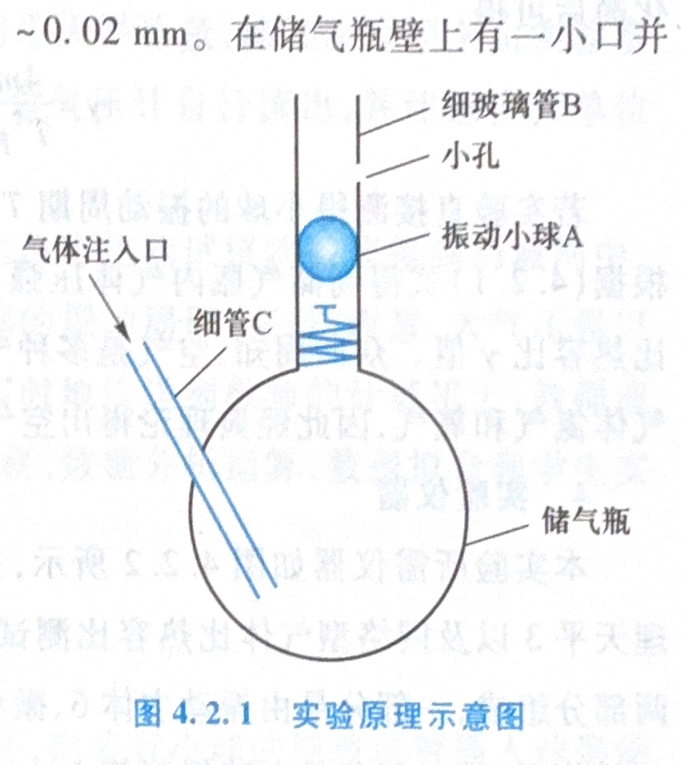
\includegraphics[width=5.2cm]{figures/heat-apparatus.png}\par
{\small 振动法装置示意图。}\end{center}
\ReportSection{实验内容}
\ReportSubsection{仪器准备与读数}
1. 检查储气瓶、细管和进气口的密封状况，调节进气量，使小球在细管内作稳定小幅振动。\par
2. 测量小球质量，用螺旋测微计在不同方位测直径五次，并记录仪器零点修正。\par
3. 记录实验始末的大气压及储气瓶容积；用计时装置测量五次振动周期，避免把多个周期的总时长误记为单周期。\par
\ReportSubsection{计算顺序}
先修正直径并求各量平均值，再计算瓶内压强和 $\gamma$；最后合成不确定度，并与室温空气参考值 $1.402$ 比较。
\ReportSection{实验仪器}
网络型气体比热容比测试仪、带小孔细玻璃管和储气瓶、螺旋测微计、电子天平、空盒气压计及计时器。记录各仪器最小分度与估计误差。
\ReportSection{数据记录处理}
小球直径（mm；修正值由后端计算）：
\begin{center}\small\renewcommand{\arraystretch}{1.35}
\begin{tabular}{|c|c|c|}\hline
序号 & 读数 & 修正后\\\hline
1 & \Field[10mm]{diameter_01} & \Field[10mm]{diameter_corrected_01}\\\hline
2 & \Field[10mm]{diameter_02} & \Field[10mm]{diameter_corrected_02}\\\hline
3 & \Field[10mm]{diameter_03} & \Field[10mm]{diameter_corrected_03}\\\hline
4 & \Field[10mm]{diameter_04} & \Field[10mm]{diameter_corrected_04}\\\hline
5 & \Field[10mm]{diameter_05} & \Field[10mm]{diameter_corrected_05}\\\hline
\end{tabular}
\end{center}
周期（s）：
\begin{center}\small\renewcommand{\arraystretch}{1.35}
\begin{tabular}{|c|c|c|}\hline
序号 & 读数 & 与均值之差\\\hline
1 & \Field[10mm]{period_01} & \Field[10mm]{period_deviation_01}\\\hline
2 & \Field[10mm]{period_02} & \Field[10mm]{period_deviation_02}\\\hline
3 & \Field[10mm]{period_03} & \Field[10mm]{period_deviation_03}\\\hline
4 & \Field[10mm]{period_04} & \Field[10mm]{period_deviation_04}\\\hline
5 & \Field[10mm]{period_05} & \Field[10mm]{period_deviation_05}\\\hline
\end{tabular}
\end{center}
\noindent 小球质量 $m=\Field{mass_g}$ g；瓶容积 $V=\Field{volume_l}$ L；
大气压始末读数 $P_{L1}=\Field{pressure_start_kpa}$ kPa，$P_{L2}=\Field{pressure_end_kpa}$ kPa。
\ReportSection{数据记录处理（续）}
\noindent 直径零点修正 $c_d=\Field{diameter_zero_mm}$ mm；直径、质量、周期、压强、容积的仪器误差依次为
$\Field{diameter_error_mm}$ mm、$\Field{mass_error_g}$ g、$\Field{period_error_s}$ s、
$\Field{pressure_error_kpa}$ kPa、$\Field{volume_error_l}$ L。
\[\bar d=(\MathField{diameter_mean_mm}\pm\MathField{diameter_mean_u_mm})\,\mathrm{mm},\quad
\bar T=(\MathField{period_mean_s}\pm\MathField{period_mean_u_s})\,\mathrm{s}.\]
\[\bar P_L=(\MathField{pressure_mean_kpa}\pm\MathField{pressure_mean_u_kpa})\,\mathrm{kPa}.\]
\[P=\MathField{pressure_inside_pa}\,\mathrm{Pa},\qquad
\gamma=\MathField{gamma_result}.\]
\[u_\gamma=\gamma\sqrt{\left(\frac{u_m}{m}\right)^2+
\left(\frac{u_V}{V}\right)^2+
\left(\frac{2u_T}{T}\right)^2+
\left(\frac{u_P}{P}\right)^2+
\left(\frac{4u_d}{d}\right)^2}
=\MathField{gamma_uncertainty}.\]
\noindent 结果：$\gamma=\MathField{gamma_result}\pm\MathField{gamma_uncertainty}$；
与参考值百分差 $\Field{gamma_error_percent}\%$。
\ReportSection{讨论与分析}
\ReportSubsection{误差来源}
直径在计算式中以四次方出现；小球直径的零点修正和重复性往往比周期末位更影响结果。若球与管壁接触、振动幅度较大，摩擦和非线性回复力会改变周期。漏气与热交换使绝热条件变差，气压记录不及时也会造成系统偏差。\par
\ReportSubsection{结果检查}
检查修正后直径是否全为正、五次周期有无明显离群、始末气压差是否异常。计算相对不确定度时各项应使用同一单位；特别注意 mm 转 m、L 转 m$^3$、kPa 转 Pa。若 $\gamma$ 与参考值偏差超过不确定度范围，应先复查密封性和直径读数。\par
\ReportSubsection{思考题}
为何应采用小幅振动？小幅振动使气体压强变化较小，绝热方程可以线性化，周期才近似与振幅无关。为何测量五次直径？球可能并非理想球体，多方向测量可暴露形状差异并估计读数分散。
\ReportSection{实验结论}
由五次振动周期和修正后的几何、气压数据得到空气比热容比 $\gamma=\MathField{gamma_result}\pm\MathField{gamma_uncertainty}$；相对参考值 $1.402$ 的百分差为 $\Field{gamma_error_percent}\%$。结果应结合密封性和直径测量条件评价。

\ReportRecord
% ===== 原始数据图片插入区 =====
\end{document}
